\documentclass[a4paper,10pt]{article}

\usepackage[a4paper, total={6in, 9in}]{geometry}
\usepackage[utf8]{inputenc}
\usepackage{amsmath}
\usepackage{amsfonts}
\usepackage{graphicx}
\usepackage[ruled,vlined]{algorithm2e}
\usepackage{hyperref}
\usepackage{cleveref}
\usepackage{color}
\usepackage{subcaption}

\author{Harry Tzovas}

\definecolor{blue1}{RGB}{44,127,184}

\newcommand{\bull}{$\bullet$}
\newcommand{\red}[1]{{\color{red}{#1}}}
\newcommand{\blue}[1]{{\color{blue1}{#1}}}
\newcommand{\mz}{\mathbb{Z}}
\newcommand{\quot}[1]{``#1''}
\newcommand{\km}{$k$-means}
\newcommand{\geo}{\textsc{Geographer}}
\newcommand{\todo}[1]{{\red{TODO}}: #1}
\newcommand{\etc}{e.t.c.\xspace}
\newcommand\noIndent[1]{
  \par\vbox{\parbox[t]{\linewidth}{#1}}
}

\graphicspath{{/home/harry/wave/figures/}{../figures/}}

\title{Refinement using PU distances and bit labels}

\begin{document}

\maketitle


\section{Local refinement with PU communication costs}

To better exploit the system architecture,
communication costs (or distance) between PUs are used when performing local refinement and a vertex
is considered for moving to another block
(vertices do not belong to PUs but blocks; to use the costs between PUs we imply the
identity mapping where block $i$ is mapped to PU $i$).
The gain is not just the cut; every edge of the cut is weighted by the communication cost 
between the two PUs. If the PUs are close, e.g., in the same compute node, this cost is low. 
If they are far, e.g., in different racks, islands etc., the cost is high.
For a general architecture we need to maintain a $p^2$ matrix for all the distances between PUs,
where $p$ is the number of PUs.

For example see \Cref{fig:lr}. In the case where we do not know the
communication costs between PUs, the squared vertex $v$ will be moved to PU 2, as this burdens the cut 
value by only 3. If we consider the communication costs between PUs as shown in the figure, 
if $v$ remain in PU 0, it contributes a cost of 
$$
cost(\Pi(v)=0) = 2 d(0,1) + 3 d(0,2)= 2\cdot 10 + 3\cdot 10 = 50
$$,
if it moves to PU 1 the cost is 
$$
cost(\Pi(v)=1) = d(0,1) + 3d(1,2) = 10 + 3\cdot 30= 100
$$,
while if it moves to PU 2, the cost is
$$
cost(\Pi(v)=2) = d(0,2)+ 2d(1,2) = 10 + 2\cdot 30 = 70
$$.
It induces less communication costs if vertex $v$ remains in PU 0.

\begin{figure}
\centering
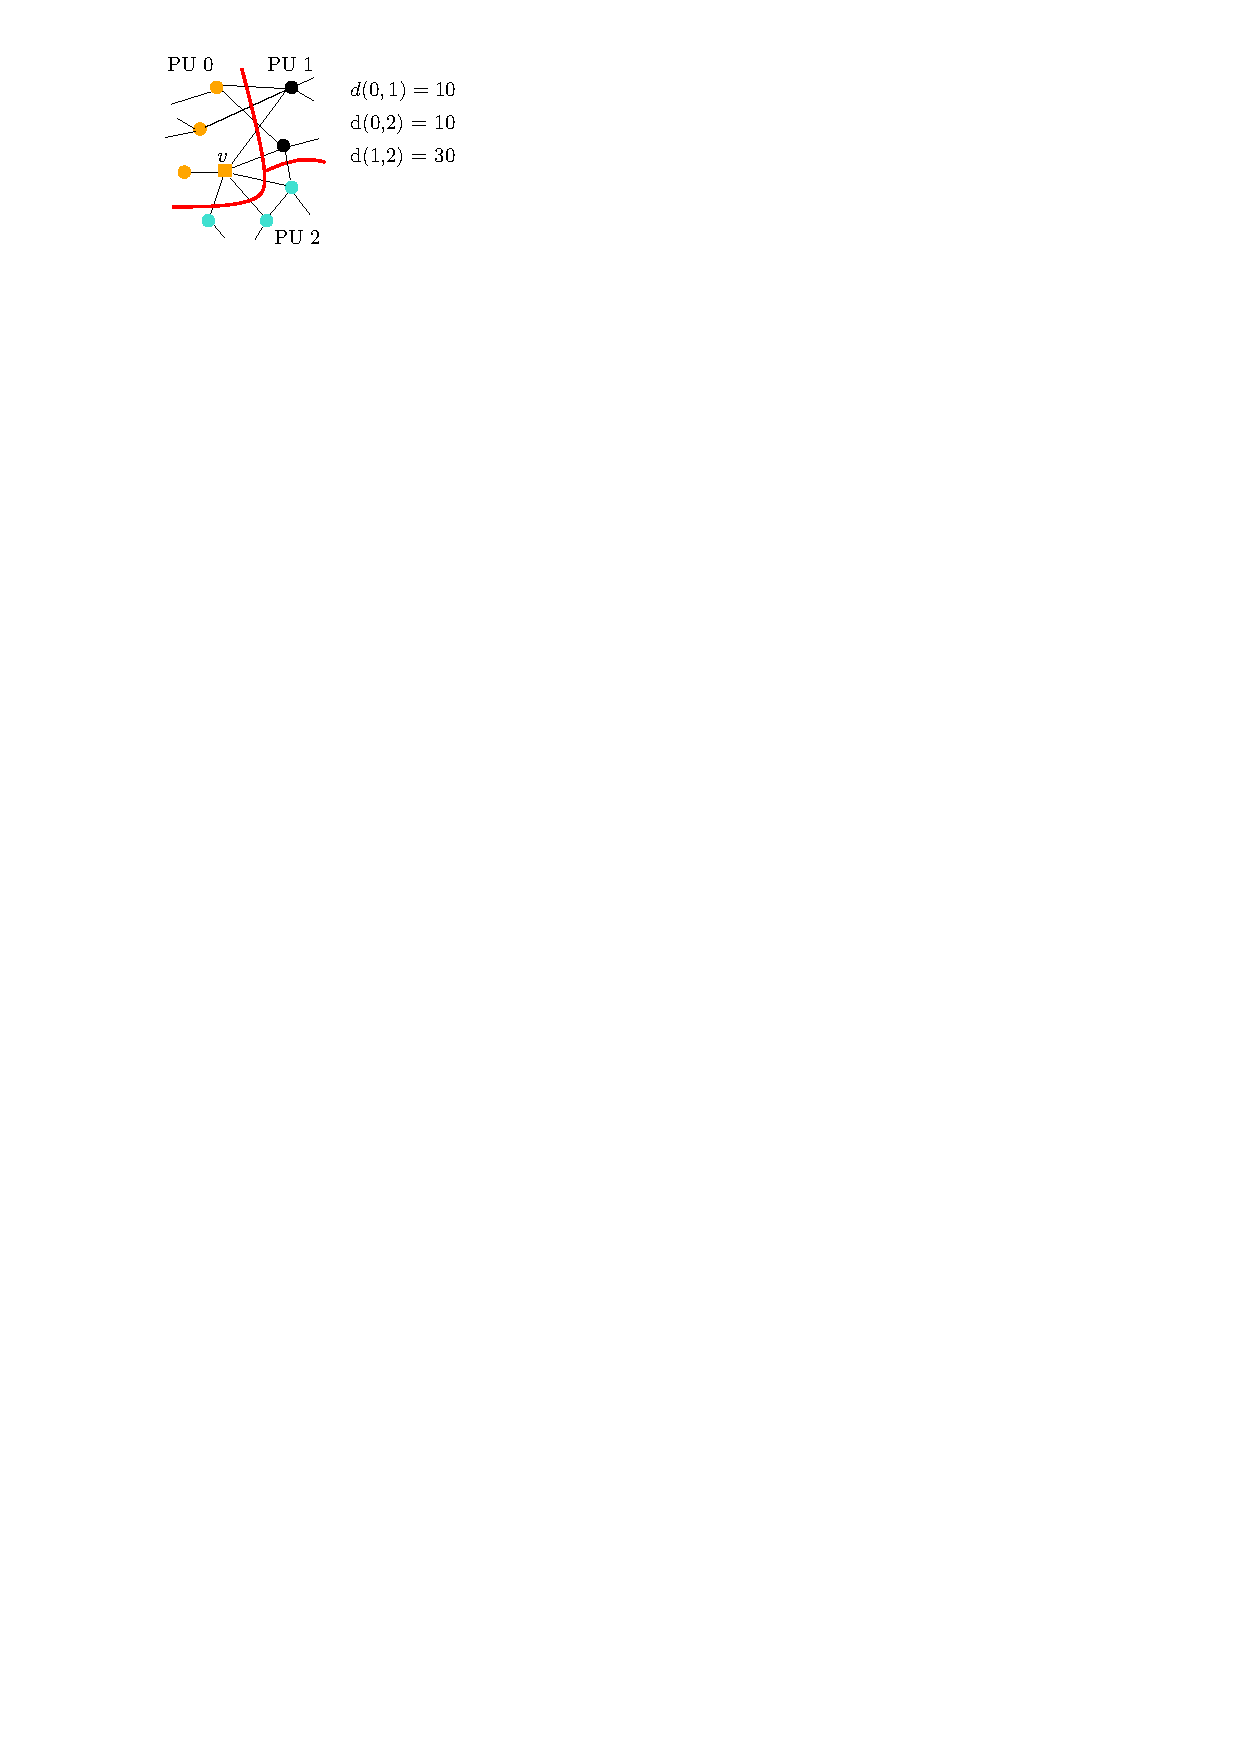
\includegraphics[scale=1.6]{local_search_PU_dist}
\caption{Red line indicates the cut. Without communication costs, the squared vertex should go to 
PU 2. If we consider the communication costs, the best PU is 1.}
\label{fig:lr}
\end{figure}


\section{Hierarchical systems}

When our architecture has a hierarchical format, we can describe it with a tree. Then, the distances
can be calculated fast on the fly without storing the distance matrix.
We will consider only trees that are balanced, with height $h$ and in each level, all nodes have
the same number of children. Also, each level has a cost $c$ which describes the communication
cost of a message if it needs to cross this level.
These trees can be described by a sequence of (number-of-children, cost) pairs
$(p_i,c_i)$
for each level $i$. The number of leaves is $\prod p_i=p$.
For example, the tree in \Cref{fig:tree} is described by the sequence $(4,500),(2,300), (3,100)$
and it has $4\cdot 2 \cdot 3 = 24$ leaves.
 
Using a tree description for the system, the PUs are the leaves of the tree and intermediate tree nodes
represent collections of PUs like CPUs, sockets, racks, \etc.
Each leaf/PU $w$ can be uniquely identified by a label $l(w)$ that describes its position in the tree.
The label has size $h$ and $l(w)[i]$ is the child position of $w$ in the $i$-th level.
For example, the leaf $w$ in \Cref{fig:tree} has label $l(w)=1,0,2$. 
The cost of communication between PUs $w$ and $z$ is $500$. The cost of communicating between $w$
and the PUs with label $1,1,\text{X}$ is $300$.

All the communication costs are stored in a vector $C$ starting from the root cost and moving down.
Naturally, the costs are in decreasing order as communication costs more if a message needs to 
go over a higher level of the tree.
For this example, $C=[500,300,100]$.
Suppose we want to find the communication cost between two PUs $w$ and $z$.
We scan their labels $l(w)$ and $l(z)$ and we find the first position they differ, say $i$.
Then, the communication cost between $w$ and $z$ is $C[i]$.  In our example, they differ in the 
first position ($l(z)=0,0,0$), so the cost is $C[0]=500$.

\begin{figure}
\centering
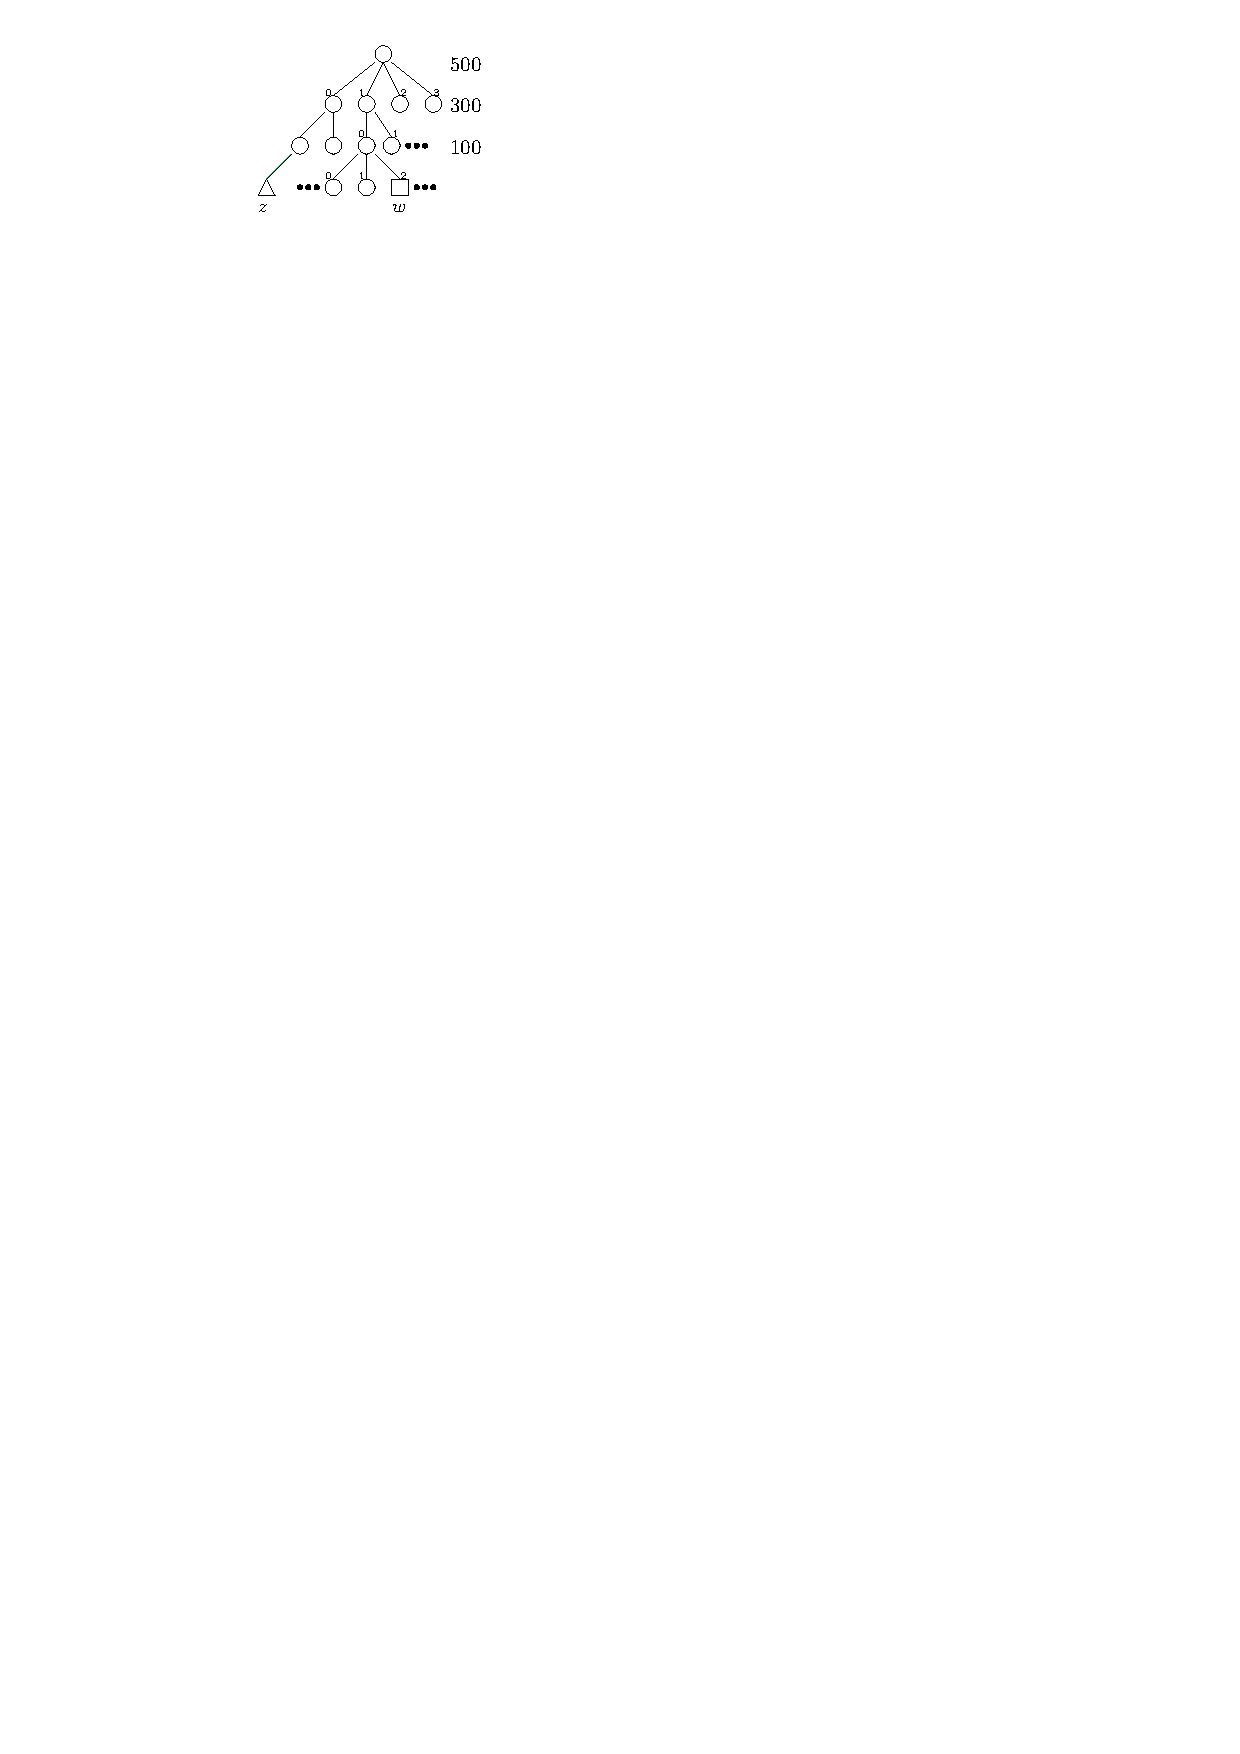
\includegraphics[scale=2]{hier_tree_system}
\caption{A tree-like system.}
\label{fig:tree}
\end{figure}

\todo{fast calculation of the cost using bit labels instead of integers}


\section{Distributed memory and integration to Geographer}

When using distributed memory, the tree structure is replicated in every PU, so no extra 
communication is needed. The problem for \geo\ is that the implementation of the local refinement
performs a number of 2-way FM steps in rounds based on an edge coloring of the communication graph.
Since the distance between PUs is symmetric, it cannot be used
for a 2-way refinement. So, the local refinement algorithm needs to be designed for k-way refinement.
This will also lift the $k=p$ restriction that is imposed by the current local refinement implementation.

%\section{Plan}

We can view this as a new local refinement algorithm in \geo\ that uses the PU distances.
For this to work, the local refinement needs to be redesigned and re-implemented to perform
a k-way refinement. We could use the current coarsening schemes and introduce bit labels
after the local refinement works. There a possibility that we have some silent assumptions
in the code or that the current code is optimized for a behavior that we will not have.
For example, we redistributed the data (using SFC) before \km\ and local refinement and
we do not know if we are going to do that now.

The first steps would be to test the competitors. This way we can have a working pipeline:
read graph and system, perform partition with competitor, evaluate solution.
And later on, we replace the competitor with \geo.


\subsection{Methodology}

\begin{enumerate}
\item (optional) Redistribute the graph so a PU own a somewhat connected subgraph.
\item Obtain initial partition on application graph ($G_a$) (other than the inherent partition implied
by the vertex labels) using a fast graph partitioner.
\item Rename vertex labels within blocks to respect PU IDs.
\item Perform HEM coarsening (locally for each PU).
\item Create coarse communication graph.
\item (optional) Renumber vertices in the communication graph such that neighboring vertices have 
small distance (reordering step using hierarchical distance of processor graph ($G_p$)).
\item Perform uncoarsening and refinement.
\end{enumerate}

%? In the SEA paper they consider $N^d(v)$ that is neighborhood of vertex $v$ with distance 
%up to $d$ and they use $d=10$.

\subsection{Refinement}
Two main ideas for the refinement process:
\begin{itemize}
\item [Move-based] Refinement process that moves a vertex $u$
  of $G_a$ to \quot{neighboring} PUs. Neighboring PUs are those that contain
  neighbor vertices $v$ of $u$ in $G_a$ ($edge (u,v) \in E(G_a)$) and those that
  %have \quot{similar} labels with the current PU and the other neighboring PUs.
  are connected with the PU of $u$ in the process graph (or its siblings in the 
  process tree).
  For the boundary nodes the direct neighbors in $G_a$
  (denoted as $N^{1}$) should be exchanged and updated between PUs after every (?) move.
  Balance constraint should be checked explicitly.

\item [Pair-based] Refinement process that swaps a vertex-pair
  $u,v$ of $G_a$. Vertex pairs are taken from a neighborhood of $d$-distance
  ($N^{d}$). For the boundary nodes, the neighborhood $N^{d}$ should be
  exchanged and updated between PUs. Balance constraint is maintained implicitly.
\end{itemize}

\end{document}
